\section{Data}
\label{sec:data}
Luminous red galaxies (LRGs) are massive galaxies that populate massive haloes, lack active star formation, and are highly biased tracers of the dark matter gravitational field \citep{postman1984ApJ...281...95P, kauffmann}. A distinct break around 4000 \AA~in the LRG spectrum is often utilized to determine their redshifts accurately. LRGs are widely targeted in previous galaxy redshift surveys \citep[see, e.g.,][]{eisenstein2001spectroscopic, prakash2016sdss}, and their clustering and redshift properties are well studied \citep[see, e.g.,][]{ross2020MNRAS.498.2354R, gilmarin2020MNRAS.498.2492G, bautista2021MNRAS.500..736B, chapman2022MNRAS.516..617C}. 

DESI is designed to collect spectra of millions of LRGs covering the redshift range $0.2<z<1.35$. DESI selects its targets for spectroscopy from the DESI Legacy Imaging Surveys, which consist of three ground-based surveys that provide photometry of the sky in the optical $g$, $r$, and $z$ bands. These surveys include the Mayall $z$-band Legacy Survey using the Mayall telescope at Kitt Peak \citep[MzLS;][]{dey2018overview}, the Beijing–Arizona Sky Survey using the Bok telescope at Kitt Peak \citep[BASS;][]{zou2017project}, and the Dark Energy Camera Legacy Survey on the Blanco 4m telescope \citep[DECaLS;][]{flaugher2015dark}. As shown in Figure \ref{fig:ng}, the BASS and MzLS programmes observed the same footprint in the North Galactic Cap (NGC) while the DECaLS programme observed both caps around the galactic plane; the BASS+MzLS footprint is separated from the DECaLS NGC at DEC $> 32.375$ degrees, although there is an overlap between the two regions for calibration purposes \citep{dey2018overview}. Additionally, the DECaLS programme integrates observations executed from the Blanco instrument under the Dark Energy Survey \citep{abbott2016dark}, which cover about $1130 \deg^{2}$ of the South Galactic Cap (SGC) footprint. The DESI imaging catalogues also integrate the $3.4$ (W1) and $4.6$ $\mu m$ (W2) infrared photometry from the Wide-Field Infrared Explorer \citep[WISE;][]{wise2010AJ....140.1868W, meisner2018RNAAS...2....1M}.  

\subsection{DESI imaging LRGs}
Our sample of LRGs is drawn from the DESI Legacy Imaging Surveys Data Release 9 \citep[DR9;][]{dey2018overview} using the color-magnitude selection criteria designed for the DESI 1\% survey \citep{desi2023sv}, described as the Survey Validation 3 (SV3) selection in more detail in \cite{zhou2022target}. The color-magnitude selection cuts are defined in the $g$, $r$, $z$ bands in the optical and $W1$ band in the infrared, as summarized in Table \ref{tab:ts}. The selection cuts vary for each imaging survey, but they are designed to achieve a nearly consistent density of approximately $800$ galaxies per square degree across a total area of roughly $14,000$ square degrees. Table \ref{tab:imaging} summarizes the mean galaxy density and area for each region. This is accomplished despite variations in survey efficiency and photometric calibration between DECaLS and BASS+MzLS. The implementation of these selection cuts in the DESI data processing pipeline is explained in \cite{myers2022}. The redshift distribution of our galaxy sample are inferred respectively from DESI spectroscopy during the Survey Validation phase \citep{desi2023sv}, and is shown via the solid curve in Figure \ref{fig:nz}. \cite{zhou2021clustering} analyzed the DESI LRG targets and found that the redshift evolution of the linear bias for these targets is consistent with a constant clustering amplitude and varies via $1/D(z)$, where $D(z)$ is the growth factor (as illustrated by the dashed red line in Figure \ref{fig:nz}). 

\begin{figure}
 \centering
 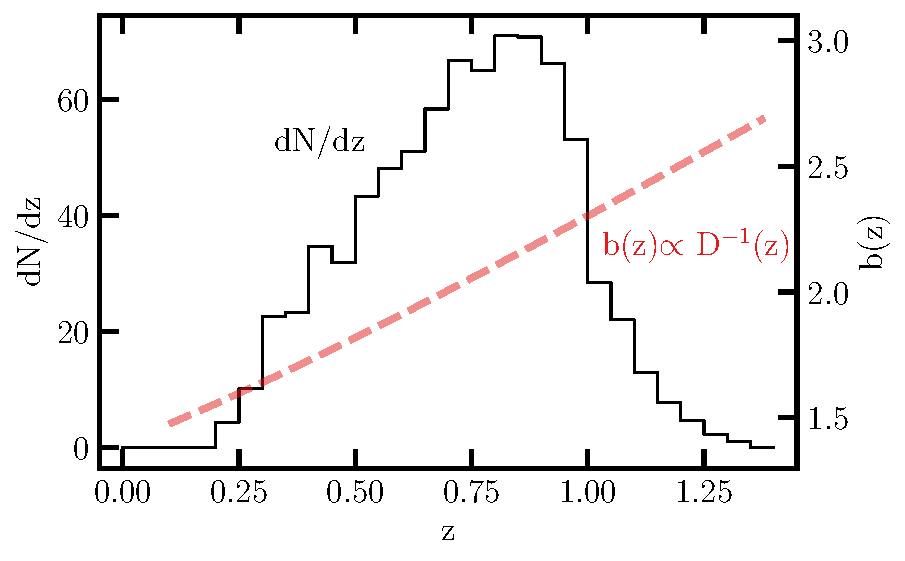
\includegraphics[width=0.5\textwidth]{figures/nz_lrg.pdf}
 \caption{The redshift distribution (solid line and vertical scale on the left) and bias evolution (dashed line and vertical scale on the right) of the DESI LRG targets. The redshift distribution is determined from DESI spectroscopy \citep{desi2023sv}. The redshift evolution of the linear bias is supported by HOD fits to the angular clustering of the DESI LRG targets \citep{zhou2021clustering}, where $D(z)$ represents the growth factor.}
 \label{fig:nz}
\end{figure}

\begin{table*}
\caption{Color-magnitude selection criteria for the DESI LRG targets \citep{zhou2022target}. Magnitudes are corrected for Galactic extinction. The z-band fiber magnitude, $z_{\rm fiber}$, corresponds to the expected flux within a DESI fiber.}\label{tab:ts}
 \centerline{%
 \begin{tabular}{lll}
 \hline
 \hline
 \textbf{Footprint} & \textbf{Criterion} &\textbf{Description}\\
 \hline
 \hline  
 & $z_{\rm fiber} < 21.7$ & Faint limit \\
  DECaLS & $z - W1 > 0.8 \times (r - z) - 0.6$ & Stellar rejection \\
 & $[(g-r >1.3)~{\rm AND}~((g-r) > -1.55*(r-W1) + 3.13)]~{\rm OR}~(r -W 1 > 1.8)$ & Remove low-z galaxies \\
 & $[(r-W1 > (W1 - 17.26)*1.8)~{\rm AND}~(r - W1 > W1 - 16.36)]~{\rm OR}~(r-W1 > 3.29)$ & Luminosity cut \\ 
 \hline
 & $z_{\rm fiber} < 21.71$ & Faint limit \\
 BASS+MzLS & $z - W1 > 0.8 \times (r - z) - 0.6$ & Stellar rejection \\
 & $[(g-r >1.34)~{\rm AND}~((g-r) > -1.55*(r-W1) + 3.23)]~{\rm OR}~(r -W 1 > 1.8)$ & Remove low-z galaxies \\
 & $[(r-W1 > (W1 - 17.24)*1.83)~{\rm AND}~(r - W1 > W1 - 16.33)]~{\rm OR}~(r-W1 > 3.39)$ & Luminosity cut \\ 
 \hline
 \end{tabular}}
\end{table*}

\begin{figure*}
 \centering
 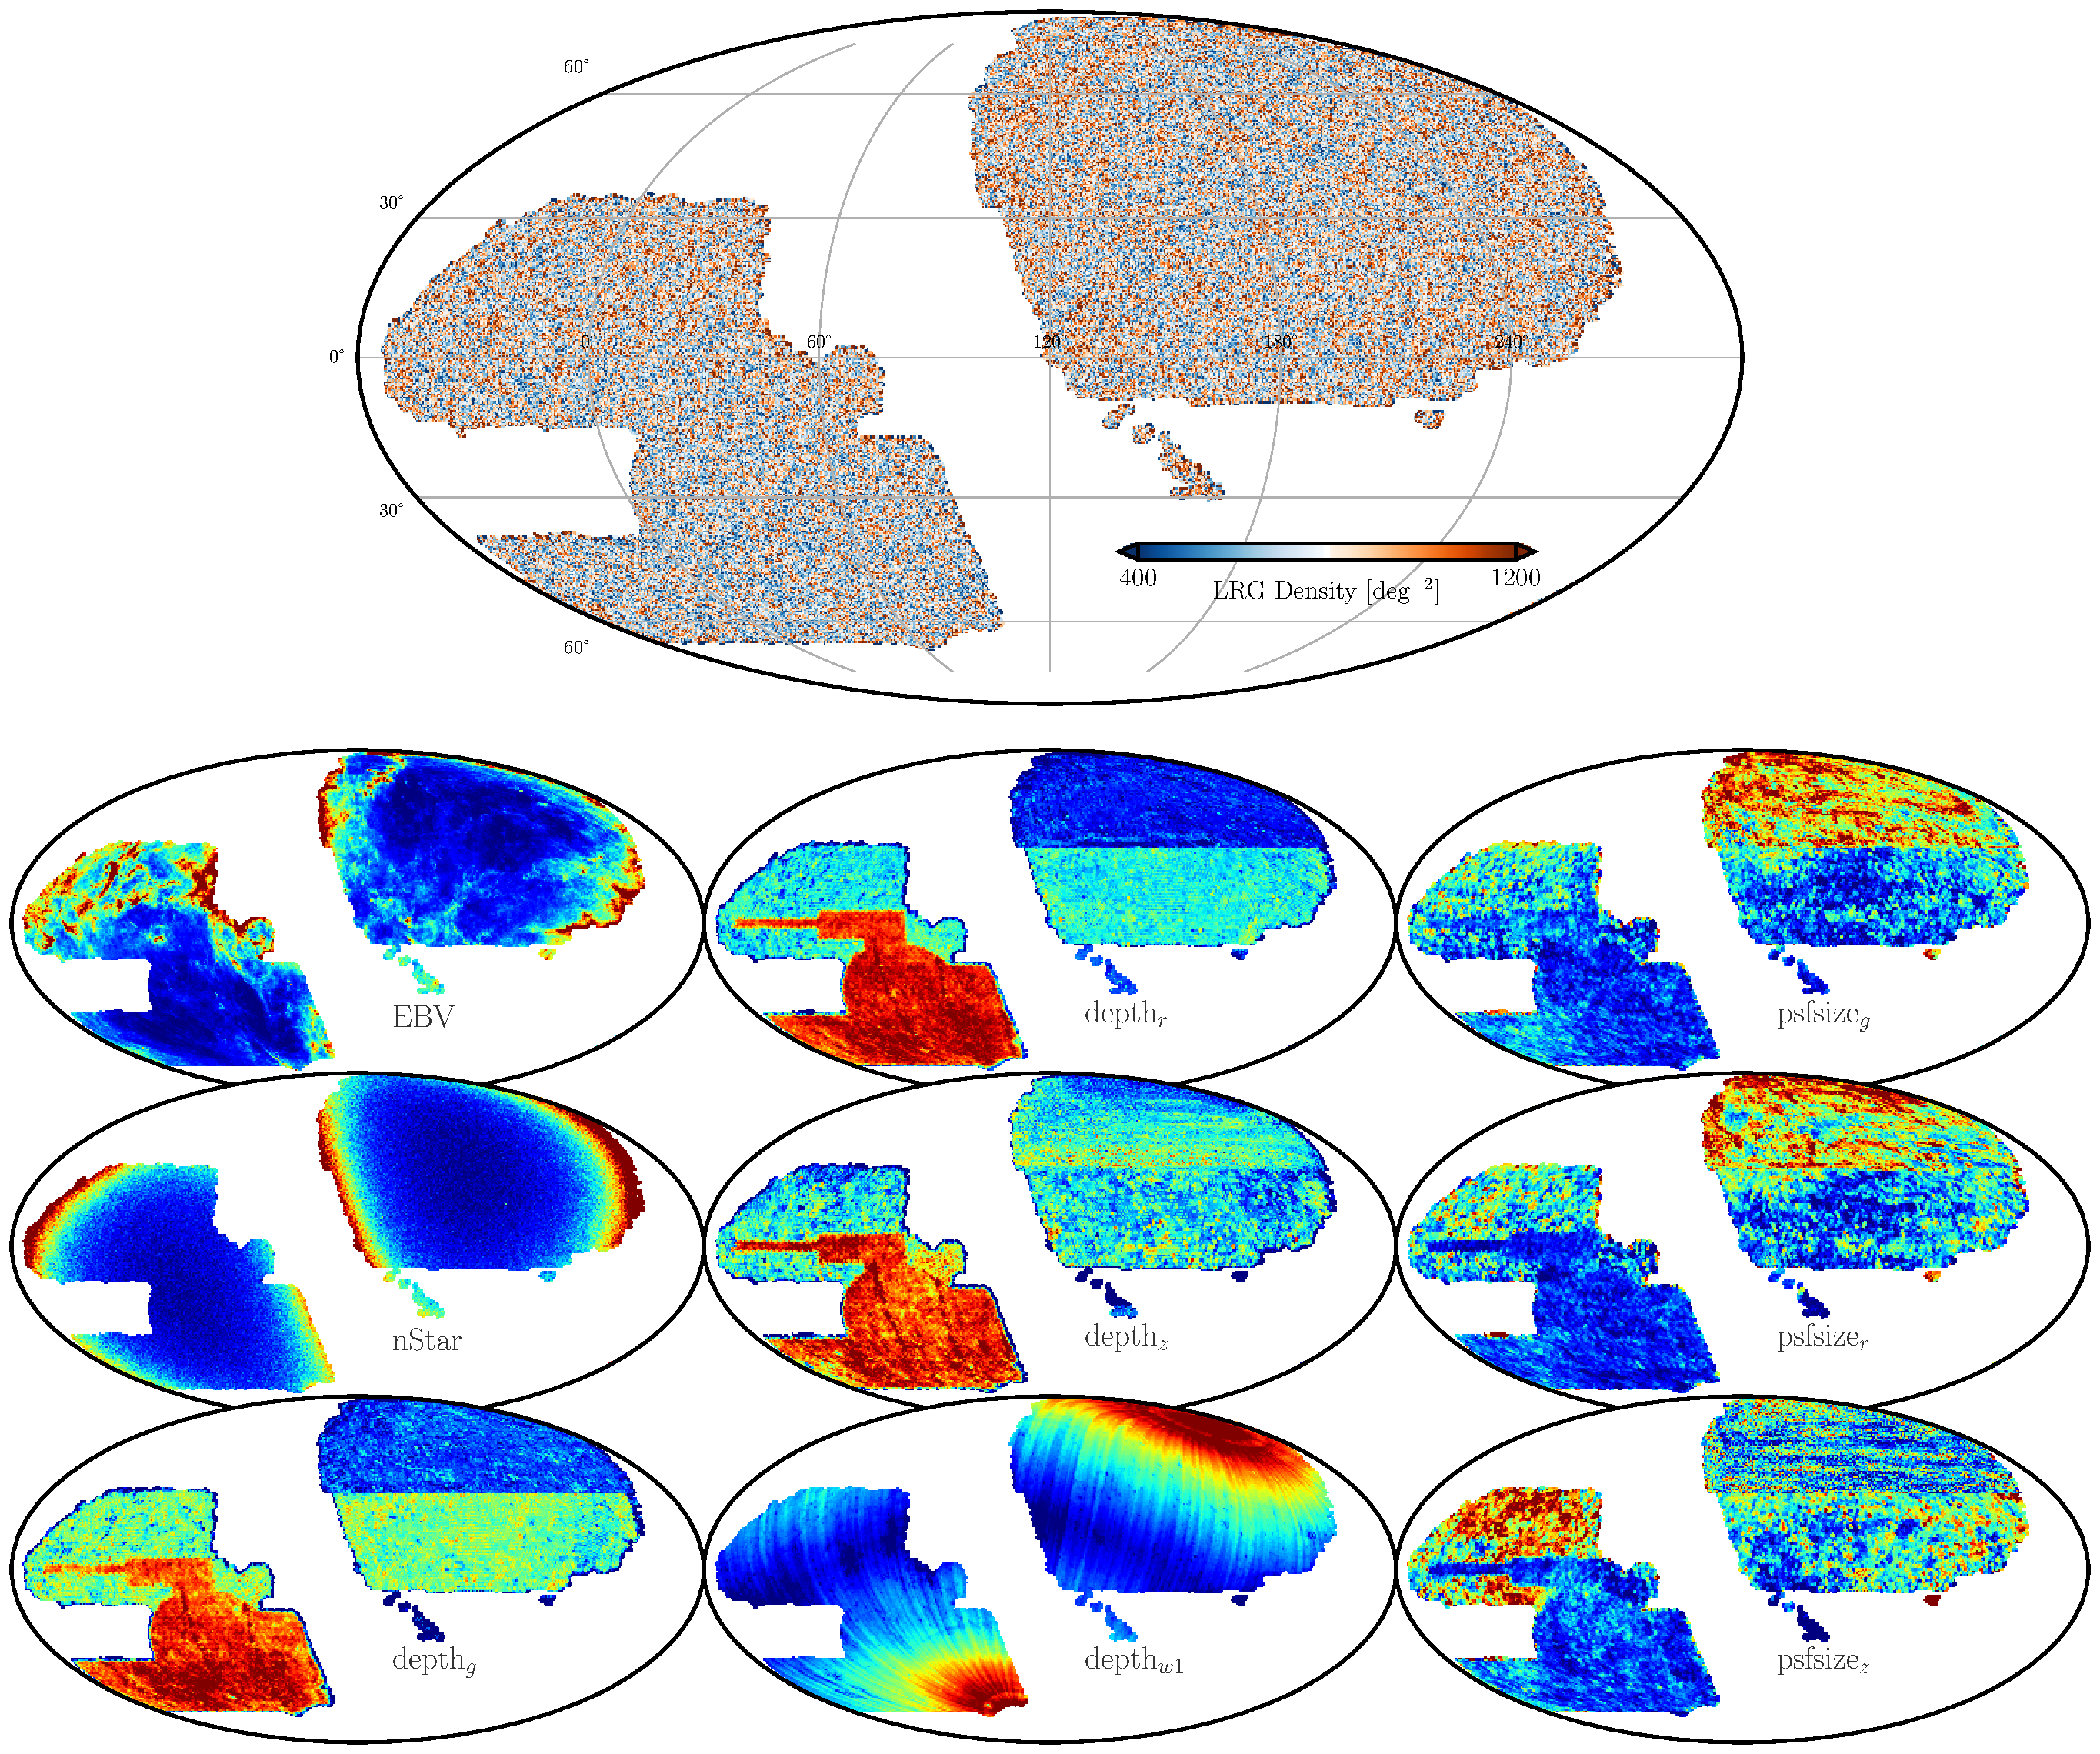
\includegraphics[width=\textwidth]{figures/dr9data.pdf}
 \caption{Top: The DESI LRG target density map before correcting for imaging systematic effects in Mollweide projection. The disconnected islands from the North footprint and parts of the South footprint with declination below $-30$ are removed from the sample for the analysis due to potential calibration issues (see text). Bottom: Mollweide projections of the imaging systematic maps (survey depth, astronomical seeing/psfsize, Galactic extinction, and local stellar density) in celestial coordinates. Not shown here are two external maps for the neutral hydrogen column density and photometric calibration, which are only employed for the robustness tests. The imaging systematic maps are colour-coded to show increasing values from blue to red.}
 \label{fig:ng}
\end{figure*}

The LRG sample is masked rigorously for foreground bright stars, bright galaxies, and clusters of galaxies\footnote{See \url{https://www.legacysurvey.org/dr9/bitmasks/} for maskbit definitions.} to further reduce stellar contamination \citep{zhou2022target}. Then, the sample is binned into \textsc{HEALPix} \citep{gorski2005healpix} pixels at $\textsc{nside}=256$, corresponding to pixels of about $0.25$ degrees on a side, to construct the 2D density map (as shown in the top panel of Figure \ref{fig:ng}). The LRG density is corrected for the pixel incompleteness and lost areas using a catalogue of random points, hereafter referred to as randoms, uniformly scattered over the footprint with the same cuts and masks applied. Moreover, the density of galaxies is matched to the randoms separately for each of the three data sections (BASS+MzLS, DECaLS North / South) so the mean density differences are mitigated (see Table \ref{tab:imaging}). The DESI LRG targets are selected brighter than the imaging survey depth limits, e.g., $g=24.4,~r=23.8,~{\rm and}~z=22.9$ for the median $5\sigma$ detection in AB mag in the DECaLS North region (Table \ref{tab:imaging}); and thus the LRG density map does not exhibit severe spurious fluctuations.

\subsubsection{Imaging systematic maps}
The effects of observational systematics in the DESI targets have been studied in great detail \cite[see, e.g.,][]{kitanidis2020imaging, zhou2021clustering, chaussidon2022angular}.  \cite{zhou2022target} has previously identified nine astrophysical properties as potential sources of imaging systematic errors in the DESI LRG targets. These imaging properties are mapped into \textsc{HEALPix} of \textsc{nside}$=256$. As illustrated by the $3\times3$ grid in the bottom panel of Figure \ref{fig:ng}, the maps include local stellar density constructed from point-like sources with a G-band magnitude in the range $12 \leq G < 17$ from the \textit{Gaia} DR2 \citep[see,][]{gaiadr2, myers2022}; Galactic extinction E[B-V] from \cite{schlegel1998maps}; survey depth (galaxy depth in $g$, $r$, and $z$ and PSF depth in W1) and astronomical seeing (i.e., point spread function, or psfsize) in $g$, $r$, and $z$. The depth maps have been corrected for extinction using the coefficients adapted from \cite{2011ApJ...737..103S}. Table \ref{tab:imaging} summarizes the median values for the imaging properties in each region. In addition to these nine maps, we consider two external maps for the neutral hydrogen column density (HI) from \cite{2016A&A...594A.116H} and photometric calibration in the z-band (CALIBZ) from \cite{desi2023sv} to further test the robustness of our analysis against unknown systematics.

\begin{table*}
\caption{Statistics for DESI imaging data. Median depths are for galaxy/point sources detected at $5\sigma$. Median psfsize values are computed with a depth-weighted average at each location on the sky.}
\begin{center}
\begin{tabular}{lccc}
\hline
\hline
    & BASS+MzLS & DECaLS North &DECaLS South \\
\hline
\hline
Mean galaxy density [deg$^{-2}$]     & 804  & 808  & 796 \\
Area [deg$^2$]                       & 4525 & 5257 & 5188 \\
Median extinction [mag]              & 0.02 & 0.03 & 0.05\\
Median stellar density [deg$^{-2}$]  & 667  & 629  & 629\\
Median $g$ galaxy depth [mag]        & 24.0 & 24.4 & 24.5 \\
Median $r$ galaxy depth [mag]        & 23.4 & 23.8 & 23.9\\
Median $z$ galaxy depth [mag]        & 23.0 & 22.9 & 23.1\\
Median $W1$ psf depth [mag]          & 21.6 & 21.4 & 21.4\\
Median $g$ psfsize [arcsec]          & 1.9  & 1.5  & 1.5\\
Median $r$ psfsize [arcsec]          & 1.7  & 1.4  & 1.3\\
Median $z$ psfsize [arcsec]          & 1.2  & 1.3  & 1.3\\
\hline
\end{tabular}
\end{center}
\label{tab:imaging}
\end{table*} 

The fluctuations in each imaging map are unique and tend to be correlated with the LRG density map. For instance, large-scale LRG density fluctuations could be caused by stellar density, extinction, or survey depth; while small scale-fluctuations could be caused by psfsize variations. Some regions of the DR9 footprint are removed from our analysis to avoid potential photometric calibration issues. These regions are either disconnected from the main footprint (e.g., the islands in the NGC with DEC $<-10$) or calibrated using different catalogues of standard stars (e.g., DEC $<-30$ in the SGC). The potential impact of not imposing these declination cuts on the LRG sample and our $\fnl$ constraints is explored in Section \ref{sec:results}. 

\begin{figure}
\centering
 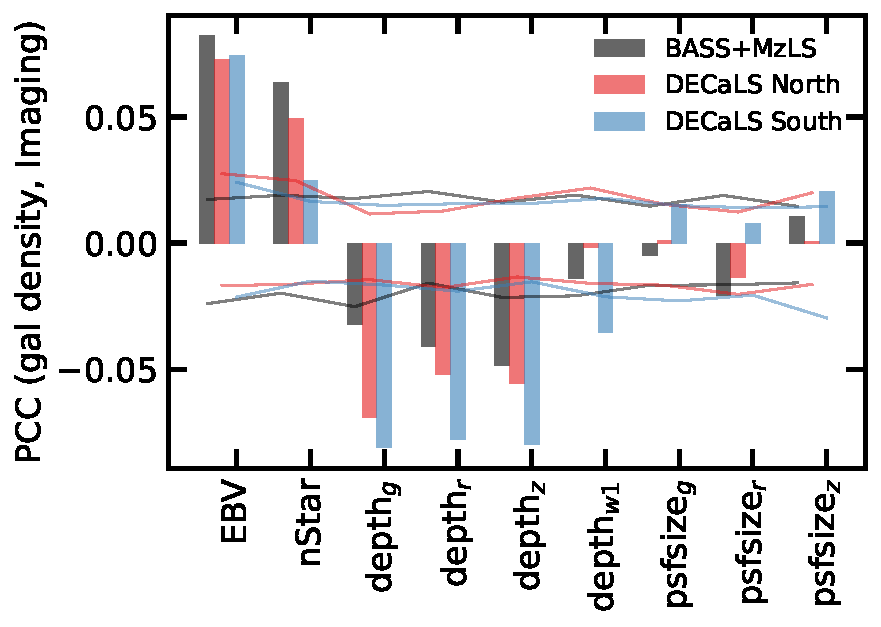
\includegraphics[width=0.45\textwidth]{figures/pcc.pdf} 
 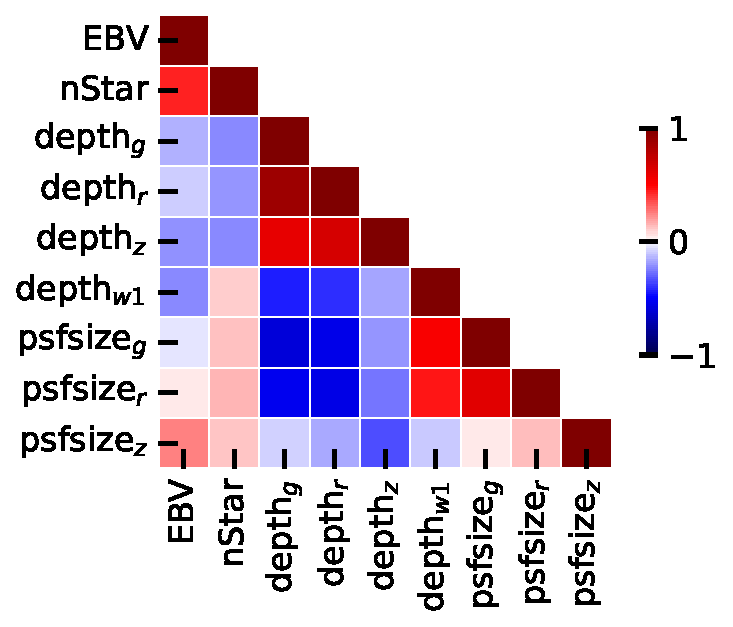
\includegraphics[width=0.45\textwidth]{figures/pccx.pdf}  
 \caption{Top: The Pearson correlation coefficient between the DESI LRG target density and imaging properties in BASS+MzLS, DECaLS North, and DECaLS South. Solid horizontal curves represent the $95\%$ confidence intervals estimated from simulations of lognormal density fields with $\fnl=0$. Bottom: The Pearson correlation matrix of imaging properties for the DESI footprint.}
 \label{fig:pcc}
\end{figure}

We employ the Pearson correlation coefficient to characterize the correlation between the galaxy density and imaging properties, which for two random variables $x$ and $y$ is given by, 
\begin{equation}
	\text{Pearson}~(x, y) = \frac{\sum (x_{i}-\bar{x})(y_{i}-\bar{y})}{\sqrt{\sum (x_{i}-\bar{x})^{2}\sum (y_{i}-\bar{y})^{2}}},
\end{equation}
where $\bar{x}$ and $\bar{y}$ represent the mean estimates of the random variables. Figure \ref{fig:pcc} shows the Pearson correlation coefficient between the DESI LRG target density map and the imaging systematics maps for the three imaging regions (DECaLS North, DECaLS South, and BASS+MzLS) in the top panel. The horizontal curves represent the $95\%$ confidence regions for no correlation and are constructed by cross-correlating 100 synthetic lognormal density fields, generated with $\fnl=0$, and the imaging systematic maps. Consistent among the different regions, there are statistically significant correlations between the LRG density and depth, extinction, and stellar density. There are less significant correlations between the LRG density and the $W1$-band depth and psfsize. The signs of the correlations imply that there are more targets where extinction is high, and less targets where depth is high. Another interpretation might be that more contaminants are targeted where depth is shallow. Figure \ref{fig:pcc} (bottom panel) shows the correlation matrix among the imaging systematic maps for the entire DESI footprint. Significant inner correlations exist among the imaging systematic maps themselves, especially between local stellar density and Galactic extinction; also, the $r$-band and $g$-band survey properties are more correlated with each other than with the $z$-band counterpart. Additionally, we compute the Spearman correlation coefficients between the LRG density and imaging systematic maps to assess whether or not the correlations are impacted by outliers in the imaging data, but find no substantial differences from Pearson.

\subsubsection{Treatment of imaging systematics}
There are several approaches for handling imaging systematic errors, broadly classified into data-driven and simulation-based modeling approaches \citep[see e.g.][]{ross2011, ashley2012MNRAS,Ross17,2012ApJ...761...14H,suchyta2016,delubac2016sdss, prakash2016sdss, Raichoor2017MNRAS.471.3955R, laurent2017clustering, Elvin18, 2018ApJ...863..110B, 2020MNRAS.495.1613R, kong2020,rezaie2021primordial,Everett_2022, chaussidon2022angular,Eggert_2023}. The general idea behind these approaches is to use the available data or simulations to learn or forward model the relationship between the observed target density and the imaging systematic maps, and to use this relationship, which is often described by a set of \textit{imaging weights}, to mitigate spurious fluctuations in the observed target density. Another techniques for reducing the effect of imaging systematics rely on cross-correlating different tracers of dark matter to ameliorate excess clustering signals, as each tracer might respond differently to a source of systematic error \citep[see, e.g.,][]{giannantonio2014improved}. These methods have their limitations and strengths \citep[see, e.g.,][for a review]{2021MNRAS.503.5061W}. In this paper, data-driven approaches, including linear multivariate regression and artificial neural networks, are applied to the data to correct for imaging systematic effects.

\textbf{Linear multivariate model}: The linear multivariate model only uses the imaging systematic maps up to the linear power to predict the number counts of the DESI LRG targets in pixel $i$,
\begin{equation}\label{eq:npred}
    N_{i} = \log ( 1 + \exp[\textbf{a}\cdot\textbf{x}_{i}+a_{0}]),
\end{equation}
where $a_{0}$ is a global offset, and $\textbf{a}\cdot\textbf{x}_{i}$ represents the inner product between the parameters, $\textbf{a}$, and the values for imaging systematics in pixel $i$, $\textbf{x}_{i}$. The Softplus functional form for $N_{i}$ is adapted to force the predicted galaxy counts to be positive \citep{dugas2001incorporating}. Then, Markov Chain Monte Carlo (MCMC) search is performed using the \textsc{emcee} package \citep{2013PASP..125..306F} to explore the parameter space by minimizing the negative Poisson log-likelihood between the actual and predicted number counts of galaxies.

Spatial coordinates are not included in $\textbf{x}_{i}$ to help avoid over-correction. As a result, the predicted number counts solely reflect the spurious density fluctuations that arise from varying imaging conditions. The number of pixels is substantially larger than the number of parameters for the linear model, and thus no training-validation-testing split is applied to the data for training the linear model. This aligns with the methodology used for training linear models in previous analyses \citep[see, e.g.,][]{zhou2022target}. The predicted galaxy counts are evaluated for each region using the marginalized mean estimates of the parameters, combined with those from other regions to cover the DESI footprint. The linear-based imaging weights are then defined as the inverse of the predicted target density, normalized to a median of unity.


\textbf{Neural network model}: Our neural network-based mitigation approach uses the implementation of fully connected feedforward neural networks from \cite{rezaie2021primordial}. With the neural network approach, $\textbf{a}\cdot\textbf{x}_{i}$ in Equation \ref{eq:npred} is replaced with $NN(\textbf{x}_{i}|\textbf{a})$, where $NN$ represents the fully connected neural network and $\textbf{a}$ denotes its parameters. The implementation, training, validation, and application of neural networks on galaxy survey data are presented in \cite{rezaie2021primordial}. We briefly summarize the methodology here. 

A fully connected feedforward neural network (also called a \textit{multi-layer perceptron}) is a type of artificial neural network where the neurons are arranged in layers, and each neuron in one layer is connected to every neuron in the next layer. The imaging systematic information flows only in one direction, from input to output. Each neuron applies a non-linear activation function (i.e., transformation) to the weighted sum of its inputs, which are the outputs of the neurons in the previous layer. The output of the last layer is the model prediction for the number counts of galaxies. Our architecture consists of three hidden layers with 20 rectifier activation functions on each layer, and a single neuron in the output layer. The rectifier is defined as ${\rm max}(0, x)$ to introduce nonlinearities in the neural network \citep{nair2010rectified}. This simple form of nonlinearity is very effective in enabling deep neural networks to learn more complex, non-linear relationships between the input imaging maps and output galaxy counts.

Compared with linear regression, neural networks potentially are more prone to over-fitting, i.e., excellent performance on training data and poor performance on validation (or test) data. Therefore, our analysis uses a training-validation-testing split to avoid over-fitting and ensure that the neural network is well-optimized. Specifically, $60\%$ of the LRG data is used for training, $20\%$ is used for validation, and $20\%$ is used for testing. The split is performed randomly aside from the locations of the pixels. We also test a geometrical split in which neighboring pixels belong to the same set of training, testing, or validation, but no significant performance difference is observed.

The neural networks are trained for up to 70 training epochs with the gradient descent \textsc{Adam} optimizer \citep{2017arXiv171105101L}, which iteratively updates the neural network parameters following the gradient of the negative Poisson log-likelihood. The step size of the parameter updates is controlled via the learning rate hyper-parameter, which is initialized with a grid search and is designed to dynamically vary between two boundary values of $0.001$ and $0.1$ to avoid local minima \citep[see again,][]{2016arXiv160803983L}. At each training epoch, the neural network model is applied to the validation set, and ultimately the model with the best performance on validation is identified and applied to the test set. The neural network models are tested on the entirety of the LRG sample with the technique of permuting the choice of the training, validation, or testing sets \citep{arlot2010survey}. With the cross-validation technique, the model predictions from the different test sets are aggregated together to form the predicted target density map into the DESI footprint. To reduce the error in the predicted number counts, we train an ensemble of 20 neural network models and average over the predictions. The imaging weights are then defined as the inverse of the predicted target density, normalized to a median of unity.



%\subsection{Characterization of remaining systematics}
%\label{ssec:characterization}
\mc{This paragraph is adapted from Section `3.4 characterization of remaining systematics' in the original manuscript, which is now partially moved to Appendix \ref{sec:systests}. The primary driver for this change was that we noticed an error in the covariances used for our validation test. The error fix revealed that the validation tests (namely mean density and cross power spectrum) presented in Section 3.4 depends on the value of fNL used in the mocks.} One potential problem that can arise in the data-driven mitigation approach is \textit{over-correction}, which occurs when the corrections applied to the data remove the clustering signal and induce additional biases in the inferred parameter of interest. The neural network approach is more prone to this issue compared to the linear approach due to its increased degrees of freedom. As illustrated in the bottom panel of Figure \ref{fig:pcc}, the significant correlations among the imaging systematic maps may pose additional challenges for modeling the spurious fluctuations in the galaxy density field. Specifically, using highly correlated imaging systematic maps increases the statistical noise in the imaging weights, which elevates the potential for over subtracting the clustering power. These over-correction effects are estimated to have a negligible impact on baryon acoustic oscillations \citep{merz2021clustering}; however, they can significantly modulate the galaxy power spectrum on large scales, and thus lead to biased $\fnl$ constraints \citep{rezaie2021primordial, mueller2022primordial}. Although not explored thoroughly, the over-correction issues could limit the detectability of primordial features in the galaxy power spectrum and that of parity violations in higher order clustering statistics \citep{beutler2019primordial, cahn2021test, philcox2022probing}. Therefore, it is crucial to develop, implement, and apply techniques to minimize and control over-correction in the hope of ensuring that the constraints are as accurate and reliable as possible; one such approach is to reduce the dimensionality of the problem. Our goal is to reduce the correlations between the DESI LRG target density and the imaging systematic maps while controlling the over-correction effect. \mr{In Appendix \ref{sec:systests}}\mout{Below}, we describe how we \mout{achieve}\mr{approach} this objective, by employing a series of simulations along with the residual systematics that we construct based on the cross power spectrum between the LRG density and imaging maps, and the mean LRG density as a function of imaging. We test different sets of the imaging systematic maps to identify the optimal set of the feature maps:
\begin{enumerate}[itemindent=*]
\item \textbf{Two maps}: Extinction, depth in z.
\item \textbf{Three maps}: Extinction, depth in z, psfsize in r.
\item \textbf{Four maps}: Extinction, depth in z, psfsize in r, stellar density.
\item \mout{\textbf{Five maps}: Extinction, depth in z, psfsize in r, neutral hydrogen density, and photometric calibration in z.}
\item \textbf{Eight maps}: Extinction, depth in $grzW1$, psfsize in $grz$.
\item \textbf{Nine maps}: Extinction, depth in $grzW1$, psfsize in $grz$, stellar density.
\item \mr{\textbf{Eleven maps}: same as Nine maps but with two additional maps; Extinction, depth in $grzW1$, psfsize in $grz$, stellar density, neutral hydrogen density, and photometric calibration in z.}
\end{enumerate}
It is imperative to note that these sets are selected prior to examining the auto power spectrum of the LRG sample and unblinding the $\fnl$ constraints, and that the auto power spectrum and $\fnl$ measurements are unblinded only after our mitigation methods passed our rigorous tests for residual systematics.

\subsection{Synthetic lognormal density fields}\label{ssec:mocks}
Density fluctuations of galaxies on large scales can be approximated with lognormal distributions \citep{coles1991, 2017MNRAS.466.1444C}. Unlike N-body simulations, simulating lognormal density fields is not computationally intensive, and allows quick and robust validation of data analysis pipelines. Lognormal simulations are therefore considered efficient for our study since the signature of local PNG appears on large-scales and small-scale clustering is not used in our analysis. The package \textsc{FLASK} \citep[Full-sky Lognormal Astro-fields Simulation Kit;][]{Xavier_2016} is employed to generate ensembles of synthetic lognormal density maps that mimic the bias, redshift, and angular distributions of the DESI LRG targets, as illustrated in Figure \ref{fig:nz} and \ref{fig:ng}. Two universes with $\fnl=0$ and $76.9$ are considered. A set of 1000 realizations is produced for every $\fnl$. The mocks are designed to match the clustering signal of the DESI LRG targets on scales insensitive to $\fnl$. The analysis adapts the fiducial BOSS cosmology \citep{2017MNRAS.470.2617A} which assumes a flat $\Lambda$CDM universe, including one massive neutrino with $m_{\nu}=0.06$ eV, Hubble constant $h = 0.68$, matter density $\Omega_{M}=0.31$, baryon density $\Omega_{b}=0.05$, and spectral index $n_{s}=0.967$. The amplitude of the matter density fluctuations on a scale of $8 h^{-1} \text{Mpc}$ is set as $\sigma_{8}=0.8225$. The same fiducial cosmology is used throughout this paper unless specified otherwise. Our robustness tests show that the none of the cosmological parameters can produce a $\fnl$-like signatures, and therefore, our analysis is not sensitive to the choice of fiducial cosmology.


\subsubsection{Contaminated mocks}
We employ the linear multivariate model (Equation \ref{eq:npred}) to introduce synthetic spurious fluctuations in the lognormal density fields, and validate our imaging systematic mitigation methods. The motivation for choosing a linear contamination model is to assess how much of the clustering signal can be removed by applying more flexible models, based on neural networks, for correcting less severe imaging systematic effects. The imaging systematic maps considered for the contamination model are extinction, depth in z, and psfsize in r. As shown in the Pearson correlation (Figure \ref{fig:pcc}) and will be discussed later in Appendix \ref{sec:systests}, the DESI LRG targets correlate strongly with these three maps. We fit for the parameters of the linear models with the MCMC process, executed separately on each imaging survey (BASS+MzLS, DECaLS North, and DECaLS South). Then, the imaging selection function for contaminating each simulation is uniquely determined by randomly drawing from the parameter space probed by MCMC, and then the results from each imaging survey are combined to form the DESI footprint. The clean density is then multiplied by the contamination model to induce systematics.  The same contamination model is used for both the $\fnl=0$ and $76.9$ simulations.

Similar to the imaging systematic treatment analysis for the DESI LRG targets, the neural network methods with various combinations of the imaging systematic maps are applied to each simulation, with and without PNG, and with and without systematics, to derive the imaging weights. Section \ref{sec:method} presents how the simulation results are incorporated to calibrate $\fnl$ biases due to over-correction. \mout{We briefly summarize two statistical tests based on the mean galaxy density contrast and the cross power spectrum between the galaxy density and the imaging systematic maps to assess the quality of the data and the significance of the remaining systematic effects} \cite[see, also,][]{rezaie2021primordial}. \mout{We calculate these statistics and compare the values to those measured from the clean mocks before looking at the auto power spectrum of the DESI LRG targets.}
